\chapter{CƠ SỞ LÝ THUYẾT VÀ CÁC CÔNG TRÌNH LIÊN QUAN}
\label{chap:lythuyet}

\section{Tổng quan về hệ thống gợi ý (Recommendation System)}
\label{sec:tongquan_rs}

\subsection{Vì sao đề tài chọn nhánh Lọc cộng tác thay vì Lọc nội dung}
\label{subsec:khainiem_rs}

Ba hướng tiếp cận chính của một hệ thống gợi ý -- Lọc dựa trên nội dung (Content-Based, dựa trên đặc tính sản phẩm và hồ sơ sở thích quá khứ của User \parencite{schafer2001commerce}), Lọc cộng tác (Collaborative Filtering -- CF, dựa trên lịch sử tương tác chung giữa nhiều User/Item \parencite{koren2009matrix, sarwar2001item}), và Lọc lai (Hybrid, kết hợp cả hai \parencite{cheng2016wide, guo2017deepfm}) -- không cạnh tranh ngang hàng trong phạm vi đề tài này, vì lựa chọn thực chất bị quyết định bởi chính \emph{những gì dữ liệu có}. Cả hai bộ dữ liệu thực nghiệm, DataCo (mục~\ref{subsec:dataco_description}) và H\&M (mục~\ref{subsec:hm_description}), chỉ cung cấp mã định danh sản phẩm, danh mục/nhãn hàng ở mức thô và lịch sử giao dịch -- không có mô tả văn bản chi tiết hay hình ảnh sản phẩm đủ phong phú để trích xuất đặc trưng nội dung có ý nghĩa. Content-Based Filtering do đó không khả thi ngay từ bước xây dựng đặc trưng đầu vào, và Hybrid cũng không có phần "nội dung" để kết hợp. Nhánh Collaborative Filtering -- vốn chỉ cần ma trận tương tác User--Item mà không đòi hỏi đặc trưng mô tả đối tượng \parencite{su2009survey} -- là lựa chọn duy nhất phù hợp với dữ liệu sẵn có, và toàn bộ phần lý thuyết còn lại của chương này tập trung vào nhánh này.

\subsection{Lọc cộng tác dựa trên bộ nhớ (Memory-based) và dựa trên mô hình (Model-based)}
\label{subsec:memory_model_based}

Xét theo cách khai thác dữ liệu tương tác, các phương pháp Lọc cộng tác được chia thành hai nhánh chính, đặt nền móng lý thuyết cho toàn bộ hướng tiếp cận Model-based mà đề tài lựa chọn.

\textbf{Lọc cộng tác dựa trên bộ nhớ (Memory-based CF)} tính toán trực tiếp độ tương đồng giữa các User hoặc Item từ ma trận tương tác thô, không qua bước học tham số trung gian, theo nguyên lý khởi nguồn của hệ thống GroupLens \parencite{resnick1994grouplens}. Với \textbf{Item-based CF} \parencite{sarwar2001item} -- kỹ thuật được Amazon triển khai thành công ở quy mô công nghiệp \parencite{linden2003amazon} -- độ tương đồng cosine giữa hai sản phẩm $i, j$ được tính theo vector cột tương tác của chúng:
\begin{equation}
    \text{sim}(i, j) = \cos(\vec{i}, \vec{j}) = \frac{\vec{i} \cdot \vec{j}}{\lVert \vec{i} \rVert \, \lVert \vec{j} \rVert}
    \label{eq:cosine_sim}
\end{equation}
Điểm dự đoán cho cặp $(u, i)$ được ước lượng bằng tổng có trọng số các đánh giá của User $u$ trên tập $k$ láng giềng gần nhất $\mathcal{N}_k(i)$:
\begin{equation}
    \hat{y}_{ui} = \frac{\sum_{j \in \mathcal{N}_k(i)} \text{sim}(i, j) \cdot y_{uj}}{\sum_{j \in \mathcal{N}_k(i)} |\text{sim}(i, j)|}
    \label{eq:itemcf_predict}
\end{equation}
Phương pháp này được sử dụng làm baseline ItemKNN trong thực nghiệm (Chương~\ref{chap:thucnghiem}). Ưu điểm là đơn giản, dễ diễn giải và không cần huấn luyện lại toàn bộ khi có tương tác mới; tuy nhiên độ phức tạp tính toán độ tương đồng theo cặp Item tăng bậc hai theo số lượng sản phẩm ($O(N^2)$), đồng thời chất lượng dự đoán suy giảm mạnh khi ma trận tương tác thưa.

\textbf{Lọc cộng tác dựa trên mô hình (Model-based CF)} không tính tương đồng trực tiếp mà học một hàm tham số hóa (Nhân tử hóa ma trận, mạng nơ-ron) để nén thông tin tương tác thành các vector biểu diễn ẩn có số chiều thấp, cho phép tổng quát hóa tốt hơn trên dữ liệu thưa và mở rộng quy mô tuyến tính theo số lượng tương tác thay vì bậc hai theo số Item \parencite{koren2009matrix, su2009survey}. Toàn bộ các mô hình MF, GMF, MLP và NeuMF trình bày từ mục~\ref{sec:cf_mf} trở đi thuộc nhánh Model-based, là hướng tiếp cận chính của đề tài.

\subsection{Vì sao bài toán buộc phải dùng phản hồi ẩn (Implicit Feedback)}
\label{subsec:feedback_types}

Về nguyên tắc, phản hồi của User có thể là phản hồi hiện (Explicit) -- điểm số đánh giá trực tiếp như rating 1--5 sao -- hoặc phản hồi ẩn (Implicit) -- suy ra gián tiếp từ hành vi như lịch sử mua hàng, lượt click \parencite{he2017ncf, rendle2009bpr}. Điểm cần nói rõ ở đây không phải là định nghĩa chung của hai khái niệm này, mà là một ràng buộc thực tế: cả dữ liệu giao dịch DataCo lẫn dữ liệu giao dịch H\&M đều không có bất kỳ cột đánh giá (rating) nào -- chỉ có bản ghi giao dịch đã xảy ra. Điều này loại bỏ hoàn toàn khả năng dùng Explicit Feedback, và buộc toàn bộ đề tài phải xây dựng tín hiệu tương tác dưới dạng nhị phân từ chính sự kiện mua hàng:
\begin{equation}
    y_{ui} = \begin{cases}
        1, & \text{nếu tồn tại giao dịch giữa User } u \text{ và Item } i \text{ trong dữ liệu} \\
        0, & \text{ngược lại}
    \end{cases}
    \label{eq:implicit_binary}
\end{equation}
Hệ quả trực tiếp của cách xây dựng nhãn này -- $y_{ui}=1$ chỉ xác nhận \emph{đã mua}, không xác nhận \emph{hài lòng}, và $y_{ui}=0$ có thể là "chưa từng biết đến sản phẩm" chứ không hẳn "không thích" \parencite{he2017ncf} -- là lý do trực tiếp khiến kỹ thuật lấy mẫu tiêu cực (Negative Sampling, mục~\ref{subsec:dynamic_sampling}) phải được thiết kế cẩn thận thay vì coi mọi cặp chưa tương tác là nhãn âm chắc chắn đúng.

\subsection{Độ thưa dữ liệu và Cold-Start: hai giới hạn định hình phạm vi đề tài}
\label{subsec:thachthuc_sparsity}

Hai thách thức kinh điển của Collaborative Filtering không chỉ là lý thuyết trừu tượng trong phạm vi đề tài này -- chúng trực tiếp định hình các quyết định về phạm vi thực nghiệm ở mục~\ref{subsec:phamvi}:
\begin{itemize}
    \item \textbf{Độ thưa dữ liệu (Data Sparsity):} Số cặp User--Item thực sự có tương tác chỉ chiếm một phần rất nhỏ trong toàn bộ ma trận $M \times N$ \parencite{koren2009matrix}. Số liệu đo được cụ thể trên hai bộ dữ liệu của đề tài (Bảng~\ref{tab:dataco_vs_hm}, Bảng~\ref{tab:kcore_hm_full}) minh họa rõ mức độ chênh lệch có thể xảy ra: mật độ 8,16\% trên DataCo (sau lọc $k$-core) nhưng chỉ 0,62\% trên lát cắt H\&M đang dùng, và giảm xuống còn 0,03\% nếu tính trên toàn bộ 889.062 người dùng ở quy mô đầy đủ -- một khoảng cách gần 300 lần giữa hai thái cực, dùng làm cơ sở định lượng cho toàn bộ phần thảo luận so sánh hai bộ dữ liệu ở Chương~\ref{chap:thucnghiem}.
    \item \textbf{Vấn đề khởi đầu lạnh (Cold-Start):} Xảy ra khi một User hoặc Item hoàn toàn mới chưa có lịch sử tương tác nào, khiến mô hình không có dữ liệu để học vector biểu diễn cho thực thể đó. Đây chính là lý do kỹ thuật (không phải lựa chọn tùy ý) khiến bước lọc $k$-core (mục~\ref{subsec:interaction_matrix}) là bắt buộc trước khi huấn luyện: mọi User/Item còn lại sau lọc đảm bảo có ít nhất $k=5$ tương tác, tức đã "ra khỏi" vùng Cold-Start theo định nghĩa trên; ngược lại, nhóm User/Item bị loại bởi $k$-core chính là nhóm Cold-Start mà đề tài xác định rõ là nằm ngoài phạm vi đánh giá định lượng (mục~\ref{subsec:phamvi}, mục~\ref{sec:pham_vi_thuc_nghiem}).
\end{itemize}

\section{Cơ sở lý thuyết về Lọc cộng tác và Nhân tử hóa ma trận}
\label{sec:cf_mf}

\subsection{Mô hình Nhân tử hóa ma trận (Matrix Factorization -- MF)}
\label{subsec:mf_model}

Nhân tử hóa ma trận (MF) chiếu cả User và Item vào một không gian đặc trưng ẩn chung có số chiều $d \ll \min(M, N)$ \parencite{koren2009matrix}. Mỗi User $u$ được biểu diễn bởi vector $p_u \in \mathbb{R}^d$ và mỗi Item $i$ bởi vector $q_i \in \mathbb{R}^d$. Mức độ tương tác dự đoán $\hat{y}_{ui}$ được tính bằng tích vô hướng:
\begin{equation}
    \hat{y}_{ui} = p_u^T q_i = \sum_{f=1}^{d} p_{uf} q_{if}
    \label{eq:mf_dot}
\end{equation}

\subsection{Hạn chế của tích vô hướng trong mô hình hóa tương tác}
\label{subsec:mf_limitations}

Tích vô hướng kết hợp các chiều đặc trưng ẩn độc lập theo dạng tuyến tính. Phép toán này không thể học được các tương tác phức tạp và phi tuyến giữa các chiều đặc trưng của User và Item, đồng thời không đủ linh hoạt để mô hình hóa chính xác sự tương đồng không gian khi vị trí tương quan của các User thay đổi \parencite{he2017ncf}.

\subsection{Tổng quát hóa MF với đặc trưng phụ trợ: Factorization Machines (FM)}
\label{subsec:fm}

Máy Nhân tử hóa (Factorization Machines -- FM) \parencite{rendle2010fm} mở rộng MF từ bài toán chỉ có hai đặc trưng định danh (User ID, Item ID) sang bài toán tổng quát với vector đặc trưng bất kỳ $x \in \mathbb{R}^n$ (có thể bao gồm ID, danh mục sản phẩm, thời gian...), mô hình hóa \emph{mọi} tương tác cặp đôi giữa các đặc trưng thông qua tích vô hướng của các vector nhân tử ẩn $v_i \in \mathbb{R}^d$:
\begin{equation}
    \hat{y}(x) = w_0 + \sum_{i=1}^{n} w_i x_i + \sum_{i=1}^{n} \sum_{j=i+1}^{n} \langle v_i, v_j \rangle \, x_i x_j
    \label{eq:fm}
\end{equation}
Khi $x$ chỉ gồm hai đặc trưng one-hot (User, Item), FM suy biến chính xác về mô hình MF ở Công thức~\eqref{eq:mf_dot}, cho thấy MF là một trường hợp riêng của FM. Đây là cơ sở lý thuyết cho các kiến trúc lai giữa thành phần tuyến tính bậc hai và mạng nơ-ron sâu như Wide \& Deep \parencite{cheng2016wide} và DeepFM \parencite{guo2017deepfm}, được tổng hợp ở mục~\ref{sec:modern_trends}.

\subsection{Tối ưu hóa xếp hạng theo cặp: Bayesian Personalized Ranking (BPR)}
\label{subsec:bpr}

Khác với cách tiếp cận Pointwise (dự đoán độc lập từng điểm $\hat{y}_{ui}$ rồi so khớp với nhãn nhị phân như MF/GMF/MLP), Bayesian Personalized Ranking (BPR) \parencite{rendle2009bpr} tối ưu hóa trực tiếp \emph{thứ hạng tương đối} theo cặp (Pairwise Ranking), xuất phát từ giả định người dùng luôn ưa thích sản phẩm đã tương tác $i$ hơn sản phẩm chưa tương tác $j$. Với mỗi bộ ba $(u, i, j)$ trong đó $i \in \mathcal{I}_u$ và $j \notin \mathcal{I}_u$, hàm mất mát BPR cực đại hóa xác suất hậu nghiệm dưới dạng:
\begin{equation}
    \mathcal{L}_{BPR} = -\sum_{(u,i,j) \in \mathcal{D}_S} \ln \sigma\left(\hat{y}_{ui} - \hat{y}_{uj}\right) + \lambda_\Theta \lVert \Theta \rVert^2
    \label{eq:bpr_loss}
\end{equation}
trong đó $\hat{y}_{ui}, \hat{y}_{uj}$ được tính theo Công thức~\eqref{eq:mf_dot} khi kết hợp với MF (tạo thành baseline BPR-MF dùng trong Chương~\ref{chap:thucnghiem}), và $\mathcal{D}_S$ là tập các bộ ba lấy mẫu. So với hàm tổn thất Binary Cross-Entropy theo hướng Pointwise được NeuMF sử dụng (Công thức~\eqref{eq:bce_loss}), mục tiêu Pairwise của BPR bám sát hơn với bản chất bài toán xếp hạng Top-K nhưng không tận dụng được các tầng phi tuyến sâu như kiến trúc NCF.

\section{Kiến trúc Mạng khuyến nghị thần kinh (Neural Collaborative Filtering -- NCF)}
\label{sec:ncf_architecture}

\subsection{Generalized Matrix Factorization (GMF)}
\label{subsec:gmf}

Generalized Matrix Factorization (GMF) là sự mở rộng của MF dưới dạng biểu diễn mạng nơ-ron \parencite{he2017ncf}, thực hiện phép nhân Element-wise (Hadamard product $\odot$) giữa vector Embedding của User $p_u^G$ và Item $q_i^G$:
\begin{equation}
    \phi^{GMF} = p_u^G \odot q_i^G
    \label{eq:gmf_hadamard}
\end{equation}
\begin{equation}
    \hat{y}_{ui}^{GMF} = \sigma \left( h^T \phi^{GMF} \right) = \sigma \left( h^T (p_u^G \odot q_i^G) \right)
    \label{eq:gmf_predict}
\end{equation}
trong đó $\odot$ là phép nhân từng phần tử, $h$ là vector trọng số lớp đầu ra, và $\sigma(x) = \frac{1}{1 + e^{-x}}$ là hàm kích hoạt Sigmoid.

\subsection{Multi-Layer Perceptron (MLP)}
\label{subsec:mlp}

Nhánh Multi-Layer Perceptron (MLP) nối vector Embedding $p_u^M$ và $q_i^M$ (Concatenation) làm đầu vào cho chuỗi các lớp mạng liên tiếp \parencite{he2017ncf}:
\begin{equation}
    z_1 = \phi_1^{MLP} = \begin{bmatrix} p_u^M \\ q_i^M \end{bmatrix}
    \label{eq:mlp_concat}
\end{equation}
\begin{equation}
    \phi_L^{MLP} = a_L \left( W_L^T \phi_{L-1}^{MLP} + b_L \right)
    \label{eq:mlp_layerL}
\end{equation}
trong đó $W_L, b_L, a_L$ lần lượt là trọng số, độ lệch (bias) và hàm kích hoạt phi tuyến (như ReLU) tại lớp thứ $L$. Cấu trúc này giúp mô hình học các tương tác phi tuyến tính phức tạp giữa đặc trưng của User và Item.

\subsection{Kiến trúc mô hình lai NeuMF}
\label{subsec:neumf_arch}

Mô hình lai NeuMF kết hợp song song hai luồng biểu diễn tuyến tính (GMF) và phi tuyến (MLP) trước lớp dự đoán cuối cùng \parencite{he2017ncf}:
\begin{equation}
    \phi^{NeuMF} = \begin{bmatrix} \phi^{GMF} \\ \phi_L^{MLP} \end{bmatrix} = \begin{bmatrix} p_u^G \odot q_i^G \\ \phi_L^{MLP} \end{bmatrix}
    \label{eq:neumf_concat}
\end{equation}
\begin{equation}
    \hat{y}_{ui} = \sigma \left( h^T \begin{bmatrix} p_u^G \odot q_i^G \\ \phi_L^{MLP} \end{bmatrix} \right)
    \label{eq:neumf_prediction}
\end{equation}

\begin{figure}[htbp]
    \centering
    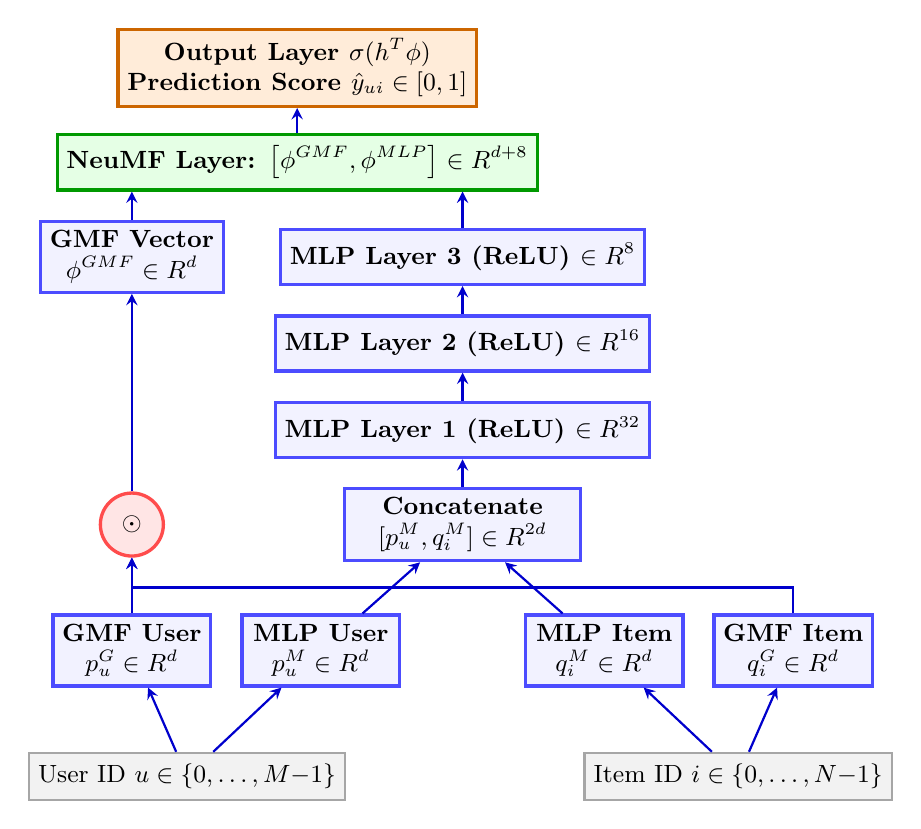
\begin{tikzpicture}[
        node distance=1.3cm,
        layer/.style={rectangle, draw=blue!70, fill=blue!5, very thick, minimum width=2.8cm, minimum height=0.7cm, font=\small\bfseries, align=center},
        op/.style={circle, draw=red!70, fill=red!10, very thick, minimum size=0.8cm, font=\small\bfseries},
        inputnode/.style={rectangle, draw=gray!70, fill=gray!10, thick, minimum width=2.2cm, minimum height=0.6cm, font=\small},
        arrow/.style={->, >=stealth, thick, color=blue!80!black}
    ]
        % Input IDs
        \node[inputnode] (user_id) at (-3.5, 0) {User ID $u \in \{0,\dots,M{-}1\}$};
        \node[inputnode] (item_id) at (3.5, 0) {Item ID $i \in \{0,\dots,N{-}1\}$};

        % Embeddings
        \node[layer, minimum width=2.0cm] (emb_ug) at (-4.2, 1.6) {GMF User\\$p_u^G \in \mathbb{R}^d$};
        \node[layer, minimum width=2.0cm] (emb_um) at (-1.8, 1.6) {MLP User\\$p_u^M \in \mathbb{R}^d$};
        \node[layer, minimum width=2.0cm] (emb_im) at (1.8, 1.6) {MLP Item\\$q_i^M \in \mathbb{R}^d$};
        \node[layer, minimum width=2.0cm] (emb_ig) at (4.2, 1.6) {GMF Item\\$q_i^G \in \mathbb{R}^d$};

        % Operations
        \node[op] (hadamard) at (-4.2, 3.2) {$\odot$};
        \node[layer, minimum width=3.0cm] (mlp_cat) at (0, 3.2) {Concatenate\\$[p_u^M, q_i^M] \in \mathbb{R}^{2d}$};

        % MLP Hidden Layers (tower thu hẹp dần, mặc định d=32 -> 2d=64)
        \node[layer, minimum width=3.0cm] (mlp_1) at (0, 4.4) {MLP Layer 1 (ReLU) $\in \mathbb{R}^{32}$};
        \node[layer, minimum width=2.6cm] (mlp_2) at (0, 5.5) {MLP Layer 2 (ReLU) $\in \mathbb{R}^{16}$};
        \node[layer, minimum width=2.2cm] (mlp_3) at (0, 6.6) {MLP Layer 3 (ReLU) $\in \mathbb{R}^{8}$};

        % GMF Vector Node
        \node[layer, minimum width=2.0cm] (gmf_out) at (-4.2, 6.6) {GMF Vector\\$\phi^{GMF} \in \mathbb{R}^d$};

        % NeuMF Concat
        \node[layer, minimum width=6.0cm, fill=green!10, draw=green!60!black] (neumf_cat) at (-2.1, 7.8) {NeuMF Layer: $\left[ \phi^{GMF}, \phi^{MLP} \right] \in \mathbb{R}^{d+8}$};

        % Output
        \node[layer, minimum width=4.0cm, fill=orange!15, draw=orange!80!black] (output) at (-2.1, 9.0) {Output Layer $\sigma(h^T \phi)$\\Prediction Score $\hat{y}_{ui} \in [0,1]$};

        % Connections
        \draw[arrow] (user_id) -- (emb_ug);
        \draw[arrow] (user_id) -- (emb_um);
        \draw[arrow] (item_id) -- (emb_im);
        \draw[arrow] (item_id) -- (emb_ig);

        \draw[arrow] (emb_ug) -- (hadamard);
        \draw[arrow] (emb_ig) -- ++(0, 0.8) -| (hadamard);

        \draw[arrow] (emb_um) -- (mlp_cat);
        \draw[arrow] (emb_im) -- (mlp_cat);

        \draw[arrow] (mlp_cat) -- (mlp_1);
        \draw[arrow] (mlp_1) -- (mlp_2);
        \draw[arrow] (mlp_2) -- (mlp_3);

        \draw[arrow] (hadamard) -- (gmf_out);

        \draw[arrow] (gmf_out) -- (neumf_cat.south -| gmf_out);
        \draw[arrow] (mlp_3) -- (neumf_cat.south -| mlp_3);

        \draw[arrow] (neumf_cat) -- (output);
    \end{tikzpicture}
    \caption{Sơ đồ kiến trúc chi tiết mô hình lai Neural Matrix Factorization (NeuMF)}
    \label{fig:neumf_architecture}
\end{figure}

\subsection{Chiến lược kết hợp: Early Fusion và Late Fusion}
\label{subsec:early_late_fusion}

Trong các kiến trúc lai kết hợp nhiều nguồn biểu diễn, thời điểm hợp nhất (fusion) các biểu diễn quyết định cách mô hình học tương tác giữa chúng \parencite{he2017ncf}.

\begin{itemize}
    \item \textbf{Early Fusion:} Các vector biểu diễn User và Item được nối (concatenate) ngay từ đầu vào, sau đó toàn bộ được đưa qua \emph{một} mạng nơ-ron chung duy nhất để học tương tác:
    \begin{equation}
        \hat{y}_{ui}^{EF} = \sigma\!\left(h^T \cdot \text{MLP}\!\left(\begin{bmatrix} p_u \\ q_i \end{bmatrix}\right)\right)
        \label{eq:early_fusion}
    \end{equation}
    trong đó $p_u, q_i$ được chia sẻ từ \emph{một} bảng Embedding chung duy nhất, khác với NeuMF ở chỗ không có nhánh nhân Element-wise tách biệt.

    \item \textbf{Late Fusion:} Mỗi nhánh (GMF, MLP) xử lý biểu diễn độc lập với bảng Embedding riêng, chỉ hợp nhất kết quả ở lớp gần cuối cùng -- đây chính là cơ chế của kiến trúc NeuMF trình bày ở mục~\ref{subsec:neumf_arch}.
\end{itemize}

Việc thực nghiệm cả hai chiến lược (Chương~\ref{chap:thietke_trienkhai} và~\ref{chap:thucnghiem}) giúp trả lời câu hỏi nghiên cứu: hợp nhất sớm hay muộn phù hợp hơn với bài toán gợi ý từ tín hiệu phản hồi ẩn dạng ID trên dữ liệu DataCo.

\subsection{Lấy mẫu tiêu cực (Negative Sampling) và hàm tổn thất Binary Cross-Entropy}
\label{subsec:negative_sampling_loss}

Do dữ liệu implicit feedback chỉ cung cấp các tương tác tích cực ($y_{ui} = 1$), kỹ thuật lấy mẫu tiêu cực (Negative Sampling) chọn ngẫu nhiên các Item mà User chưa từng tương tác để gán nhãn tiêu cực ($y_{ui} = 0$), theo giao thức chuẩn của He và cộng sự \parencite{he2017ncf}.

Hàm tổn thất Binary Cross-Entropy (BCE) được áp dụng để tối ưu hóa toàn bộ tham số mô hình:
\begin{equation}
    \mathcal{L}_{BCE} = -\sum_{(u, i) \in \mathcal{Y} \cup \mathcal{Y}^-} \left[ y_{ui} \log \hat{y}_{ui} + (1 - y_{ui}) \log (1 - \hat{y}_{ui}) \right]
    \label{eq:bce_loss}
\end{equation}
trong đó $\mathcal{Y}$ là tập tương tác tích cực và $\mathcal{Y}^-$ là tập tương tác tiêu cực được lấy mẫu.

\section{Xu hướng nghiên cứu hiện đại trong hệ thống gợi ý học sâu}
\label{sec:modern_trends}

Kiến trúc NCF/NeuMF \parencite{he2017ncf} công bố năm 2017 mở ra làn sóng thay thế tích vô hướng bằng hàm học được, nhưng lĩnh vực hệ thống gợi ý sau đó tiếp tục phát triển theo nhiều hướng song song. Mục này hệ thống hóa các hướng nghiên cứu chính giai đoạn 2016--2024, làm cơ sở xác định vị trí đóng góp của đề tài (mục~\ref{sec:khoangtrong_nghiencuu}) và định hướng phát triển tương lai (Chương~\ref{chap:ketluan}).

\subsection{Mô hình học sâu dựa trên đặc trưng tương tác (Feature-rich Deep CTR Models)}
\label{subsec:deep_ctr}

Nhóm mô hình dự đoán tỷ lệ nhấp chuột (Click-Through Rate -- CTR) mở rộng bài toán gợi ý sang không gian đặc trưng phong phú hơn cặp (User ID, Item ID). Wide \& Deep Learning \parencite{cheng2016wide} kết hợp song song một nhánh tuyến tính rộng (Wide) để ghi nhớ (memorization) các tổ hợp đặc trưng tường minh và một nhánh MLP sâu (Deep) để khái quát hóa (generalization); DeepFM \parencite{guo2017deepfm} thay thế nhánh Wide bằng Factorization Machines (mục~\ref{subsec:fm}) để loại bỏ nhu cầu kỹ nghệ đặc trưng thủ công. Deep Interest Network (DIN) \parencite{zhou2018din} tiến xa hơn bằng cơ chế Attention, gán trọng số động cho từng sản phẩm trong lịch sử hành vi của User tùy theo mức độ liên quan với Item ứng viên đang được xếp hạng, thay vì biểu diễn toàn bộ lịch sử bằng một vector cố định như MLP truyền thống. Điểm chung của nhóm này là yêu cầu đặc trưng phụ trợ (danh mục, thuộc tính) phong phú hơn nhiều so với tín hiệu ID thuần túy mà NeuMF sử dụng.

\subsection{Kiến trúc hai tháp (Two-Tower) cho truy hồi quy mô lớn}
\label{subsec:two_tower}

Trong các hệ thống công nghiệp có hàng triệu Item (ví dụ YouTube DNN \parencite{covington2016youtube}), việc xếp hạng đầy đủ mọi cặp (User, Item) bằng mạng hợp nhất sớm là bất khả thi về mặt tính toán. Kiến trúc hai tháp (Two-Tower) mã hóa User và Item thành hai vector độc lập qua hai mạng riêng biệt \emph{không tương tác với nhau cho đến bước cuối}, cho phép tính trước (pre-compute) và lập chỉ mục vector Item bằng các cấu trúc tìm kiếm lân cận gần đúng (Approximate Nearest Neighbor) để truy hồi (retrieval) hàng nghìn ứng viên trong thời gian mili-giây, trước khi đưa qua một mô hình xếp hạng (ranking) tinh hơn ở tầng sau. Về mặt cấu trúc, nhánh MLP của NeuMF với hai bảng Embedding độc lập cho User/Item (mục~\ref{subsec:embedding_design}) chia sẻ nguyên lý tương tự cấp độ biểu diễn, nhưng khác Two-Tower ở chỗ vẫn hợp nhất và học phi tuyến trên toàn bộ ma trận tương tác thay vì tối ưu cho truy hồi rời rạc quy mô lớn.

\subsection{Gợi ý theo chuỗi hành vi (Sequential và Session-based Recommendation)}
\label{subsec:sequential_rec}

Một hạn chế cố hữu của NeuMF và các mô hình MF là coi lịch sử tương tác của User như một \emph{tập hợp không thứ tự}, bỏ qua trình tự thời gian phát sinh hành vi. Hướng nghiên cứu Sequential/Session-based Recommendation khắc phục điều này bằng cách mô hình hóa chuỗi $(i_1, i_2, \dots, i_t)$ để dự đoán sản phẩm tiếp theo $i_{t+1}$:
\begin{itemize}
    \item \textbf{GRU4Rec} \parencite{hidasi2016gru4rec} là công trình tiên phong dùng mạng hồi quy có cổng (Gated Recurrent Unit) để mã hóa phiên duyệt web thành trạng thái ẩn, dự đoán phân phối xác suất trên toàn bộ danh mục cho lượt click tiếp theo.
    \item \textbf{SASRec} \parencite{kang2018self} thay thế cơ chế hồi quy bằng Self-Attention một chiều (causal), cho phép mô hình học trọng số phụ thuộc linh hoạt giữa các sản phẩm ở vị trí xa nhau trong chuỗi mà không bị giới hạn bởi \emph{vanishing gradient} như RNN, đạt cân bằng tốt giữa mô hình Markov bậc thấp và RNN.
    \item \textbf{BERT4Rec} \parencite{sun2019bert4rec} áp dụng kiến trúc Transformer hai chiều (Bidirectional) theo phong cách BERT, huấn luyện bằng mục tiêu Cloze (che ngẫu nhiên một số vị trí trong chuỗi và dự đoán lại), giúp khai thác ngữ cảnh từ cả hai phía thay vì chỉ chiều quá khứ như SASRec.
\end{itemize}
Hướng tiếp cận này phù hợp nhất với dữ liệu có tính phiên rõ rệt (streaming, xem video, duyệt web); trên dữ liệu DataCo Supply Chain, tần suất giao dịch của mỗi User thưa và không có mốc thời gian phiên rõ ràng -- tuy nhiên, thay vì suy đoán chủ quan là "không phù hợp" rồi bỏ qua, đề tài vẫn \textbf{cài đặt và thực nghiệm SASRec} trên cả DataCo lẫn H\&M để có bằng chứng định lượng khách quan (thiết kế chi tiết mục~\ref{subsec:sasrec_design}, số liệu Chương~\ref{chap:thucnghiem}).

\subsection{Học biểu diễn trên đồ thị (Graph-based Collaborative Filtering)}
\label{subsec:graph_cf}

Ma trận tương tác User--Item có thể biểu diễn tự nhiên dưới dạng đồ thị hai phía (bipartite graph). Neural Graph Collaborative Filtering (NGCF) \parencite{wang2019ngcf} khai thác cấu trúc này bằng cách lan truyền (propagate) tín hiệu Embedding qua nhiều bước lan truyền láng giềng (giống mạng nơ-ron đồ thị -- Graph Convolutional Network), giúp vector User/Item mã hóa được cả tín hiệu tương tác bậc cao (\textit{high-order connectivity}) chứ không chỉ tương tác trực tiếp như MF. LightGCN \parencite{he2020lightgcn} đơn giản hóa NGCF bằng cách loại bỏ các phép biến đổi tuyến tính và hàm kích hoạt phi tuyến -- vốn được chứng minh là dư thừa và gây khó huấn luyện trong bài toán CF thuần túy -- chỉ giữ lại phép lan truyền tuyến tính:
\begin{equation}
    e_u^{(k+1)} = \sum_{i \in \mathcal{N}_u} \frac{1}{\sqrt{|\mathcal{N}_u|}\sqrt{|\mathcal{N}_i|}} e_i^{(k)}, \qquad
    e_u^{*} = \sum_{k=0}^{K} \alpha_k \, e_u^{(k)}
    \label{eq:lightgcn}
\end{equation}
trong đó $\mathcal{N}_u$ là tập Item lân cận của User $u$ trong đồ thị và $e_u^{*}$ là biểu diễn cuối cùng, tổng hợp có trọng số qua $K$ tầng lan truyền ($\alpha_k = 1/(K{+}1)$, trung bình cộng đều theo đúng đề xuất gốc). Dữ liệu chuỗi cung ứng DataCo vốn có độ thưa cao -- bối cảnh mà tín hiệu bậc cao qua đồ thị đã được chứng minh mang lại cải thiện đáng kể so với MF/NCF truyền thống -- nên LightGCN \textbf{đã được cài đặt và thực nghiệm} trong đề tài này, không còn dừng ở mức khảo sát lý thuyết: chi tiết thiết kế ở mục~\ref{subsec:lightgcn_design}, số liệu thực nghiệm đối chiếu trực tiếp với GMF/MLP/NeuMF ở Chương~\ref{chap:thucnghiem}.

\subsection{Học tự giám sát, sinh biểu diễn xác suất và mô hình ngôn ngữ lớn}
\label{subsec:ssl_llm}

Ba hướng nghiên cứu gần đây (2018--2024) tiếp tục định hình lại bài toán gợi ý:
\begin{itemize}
    \item \textbf{Biến phân tự mã hóa (VAE) cho CF:} Mult-VAE \parencite{liang2018multvae} mô hình hóa toàn bộ vector tương tác của một User như một phân phối đa thức (multinomial) được sinh ra từ biến ẩn Gauss, tối ưu hóa qua cận dưới biến phân (ELBO) thay vì tối ưu điểm-đến-điểm như NeuMF.
    \item \textbf{Học tự giám sát (Self-Supervised Learning):} Self-supervised Graph Learning (SGL) \parencite{wu2021sgl} bổ sung một tác vụ phụ trợ đối chiếu (contrastive) giữa các góc nhìn augmentation khác nhau của cùng một đồ thị tương tác, giúp cải thiện tính vững (robustness) của biểu diễn trước dữ liệu thưa và nhiễu -- một hướng đang được tích hợp rộng rãi vào các mô hình Graph-based CF hiện đại.
    \item \textbf{Mô hình ngôn ngữ lớn và gợi ý sinh (LLM-based / Generative Recommendation):} Làn sóng nghiên cứu 2023--2024 định hình lại bài toán gợi ý theo hướng sinh chuỗi: TIGER \parencite{rajput2023tiger} mã hóa mỗi Item thành một chuỗi token ngữ nghĩa (Semantic ID) rồi huấn luyện một mô hình sinh kiểu Transformer để sinh trực tiếp token định danh Item tiếp theo, thay vì chấm điểm và xếp hạng toàn bộ danh mục; khảo sát của Wu và cộng sự \parencite{wu2023survey_llm4rec} tổng hợp toàn diện việc khai thác tri thức và khả năng suy luận ngôn ngữ tự nhiên của LLM (GPT, LLaMA...) cho các tác vụ gợi ý, từ tăng cường đặc trưng, diễn giải kết quả đến gợi ý hội thoại (Conversational Recommendation).
    \item \textbf{Mô hình khuếch tán (Diffusion Models) cho gợi ý:} Song song với hướng LLM, một hướng nghiên cứu sinh (generative) khác nổi lên gần đây (2024--2025) là ứng dụng mô hình khuếch tán -- vốn đã chứng minh hiệu quả trong sinh ảnh -- vào bài toán gợi ý. Theo khảo sát của Wei và Fang \parencite{wei2025diffusion}, ý tưởng cốt lõi là học một quá trình khử nhiễu (denoising) dần từ một phân phối nhiễu ngẫu nhiên về phân phối tương tác thực của User, cho phép mô hình hóa được tính đa phương thức (multi-modal) trong sở thích người dùng -- điều mà các mô hình Pointwise như GMF/MLP/NeuMF (vốn chỉ dự đoán một điểm số $\hat{y}_{ui}$ duy nhất cho mỗi cặp) không biểu diễn được. Đây là hướng còn rất mới, chưa được kiểm chứng rộng rãi trên dữ liệu thương mại điện tử/chuỗi cung ứng dạng bảng (tabular) như DataCo.
\end{itemize}
Cả hai hướng LLM-based và Diffusion-based đều là những hướng nghiên cứu tiên tiến nhất tính đến thời điểm thực hiện đề tài, nhưng đòi hỏi tài nguyên tính toán và dữ liệu văn bản/ngữ cảnh phong phú vượt ngoài phạm vi dữ liệu giao dịch dạng ID của DataCo.

Khảo sát tổng quan của Zhang và cộng sự \parencite{zhang2019deeplearningsurvey} xác nhận NCF/NeuMF thuộc nhóm \emph{Neural Collaborative Filtering} nền tảng, là tiền đề trực tiếp cho phần lớn hướng phát triển kể trên; khảo sát cập nhật hơn của Li và cộng sự \parencite{li2024dnncf} (tháng 12/2024) hệ thống hóa lại toàn bộ các kiến trúc mạng nơ-ron sâu (MLP, CNN, RNN, GNN, Autoencoder, GAN) đã và đang được tích hợp vào Collaborative Filtering, xác nhận rằng nhánh MLP/GMF theo tinh thần NCF vẫn là một trong các thành phần kiến trúc nền tảng được sử dụng phổ biến nhất trong các hệ thống lai hiện đại, dù không còn là hướng tiên phong. Điều này củng cố lựa chọn của đề tài: NeuMF vẫn là một kiến trúc \emph{có cơ sở lý thuyết vững chắc và được công nhận rộng rãi} để làm nền tảng nghiên cứu, dù không phải là kiến trúc mới nhất.

Trong phạm vi đề tài, NeuMF được lựa chọn làm kiến trúc trọng tâm (thay vì các hướng mới hơn như Graph-based, Sequential hay LLM/Diffusion-based) vì ba lý do cụ thể: \textit{(i) Đặc điểm dữ liệu:} DataCo chỉ cung cấp tín hiệu ID và giá trị đơn hàng, chưa có văn bản/hình ảnh mô tả sản phẩm phong phú để khai thác đặc trưng đa phương thức hay LLM, và không có mốc thời gian phiên (session) rõ ràng để áp dụng trực tiếp mô hình tuần tự (mục~\ref{subsec:sequential_rec}); \textit{(ii) Mục tiêu khoa học của đề tài:} kiến trúc hai nhánh GMF/MLP tách biệt cho phép thực hiện Ablation Study kiểm soát chặt chẽ từng thành phần (mục~\ref{subsec:ablation}) -- điều khó thực hiện tương đương với các kiến trúc End-to-End phức tạp hơn như Graph Neural Network nhiều tầng hay mô hình sinh dựa trên Transformer; \textit{(iii) Ràng buộc thực tế về hạ tầng tính toán:} toàn bộ thực nghiệm được chạy trên CPU phổ thông (mục~\ref{sec:exp_config}), trong khi các hướng LLM-based/Diffusion-based đòi hỏi GPU và tài nguyên tính toán vượt xa phạm vi một đề tài học thuật ở quy mô này. Ba lý do này nhất quán với khoảng trống nghiên cứu được xác định ở mục~\ref{sec:khoangtrong_nghiencuu}.

\section{Các chỉ số đánh giá hệ thống gợi ý Top-K}
\label{sec:metrics}

\begin{itemize}
    \item \textbf{Hit Ratio at K (HR@K):} Đo tỷ lệ mẫu kiểm thử tích cực xuất hiện trong danh sách Top-$K$ gợi ý, theo giao thức Leave-One-Out của He và cộng sự \parencite{he2017ncf}:
    \begin{equation}
        \text{HR@K} = \frac{1}{|\mathcal{U}_{test}|} \sum_{u \in \mathcal{U}_{test}} \mathbb{I}\left( \text{Rank}(u, i_{test}) \le K \right)
        \label{eq:hr_k}
    \end{equation}

    \item \textbf{Normalized Discounted Cumulative Gain at K (NDCG@K):} Đánh giá vị trí thứ tự xuất hiện của sản phẩm kiểm thử, theo định nghĩa gốc của Järvelin và Kekäläinen \parencite{jarvelin2002}:
    \begin{equation}
        \text{NDCG@K} = \frac{\text{DCG@K}}{\text{IDCG@K}}, \quad \text{với } \text{DCG@K} = \sum_{j=1}^{K} \frac{2^{rel_j} - 1}{\log_2(j + 1)}
        \label{eq:ndcg_k}
    \end{equation}
    trong đó $rel_j \in \{0, 1\}$ là mức độ liên quan tại vị trí $j$, và $\text{IDCG@K}$ là giá trị DCG lý tưởng nhất.

    \item \textbf{Precision@K và Recall@K:} Precision@K đo tỷ lệ gợi ý đúng trong $K$ sản phẩm; Recall@K đo tỷ lệ tìm lại được các sản phẩm tích cực của người dùng.
\end{itemize}

\subsection{Các chỉ số đánh giá ngoài độ chính xác (Beyond-Accuracy Metrics)}
\label{subsec:beyond_accuracy}

Chỉ tối ưu HR@K/NDCG@K có thể khiến mô hình thiên lệch về việc luôn gợi ý các sản phẩm phổ biến nhất (\textit{popularity bias}), vốn dễ trúng nhưng ít giá trị cá nhân hóa. Để đánh giá toàn diện hơn, đề tài bổ sung nhóm chỉ số ngoài độ chính xác, làm cơ sở lý thuyết cho phân tích Popular/Long-tail ở mục~\ref{subsec:longtail_results}:
\begin{itemize}
    \item \textbf{Catalog Coverage:} Tỷ lệ số sản phẩm khác nhau từng xuất hiện trong danh sách gợi ý của toàn bộ User trên tổng số sản phẩm trong danh mục:
    \begin{equation}
        \text{Coverage} = \frac{\left| \bigcup_{u \in \mathcal{U}} \text{Rec}_K(u) \right|}{N}
        \label{eq:coverage}
    \end{equation}
    Coverage thấp cho thấy mô hình chỉ khai thác một phần nhỏ danh mục sản phẩm dù độ chính xác có thể vẫn cao.
    \item \textbf{Novelty (Self-Information):} Đo mức độ mới lạ trung bình của các sản phẩm được gợi ý, dựa trên thông tin tự thân (self-information) theo định nghĩa của Vargas và Castells \parencite{vargas2011novelty}:
    \begin{equation}
        \text{Novelty} = \frac{1}{|\mathcal{U}|\,K}\sum_{u \in \mathcal{U}} \sum_{i \in \text{Rec}_K(u)} -\log_2 P(i)
        \label{eq:novelty}
    \end{equation}
    trong đó $P(i)$ là tần suất xuất hiện của Item $i$ trong tập huấn luyện. Sản phẩm càng hiếm gặp thì $-\log_2 P(i)$ càng lớn, do đó điểm Novelty cao đồng nghĩa mô hình gợi ý đa dạng, ít thiên về sản phẩm đại trà.
    \item \textbf{Head Rate (Tỷ lệ thiên lệch phổ biến):} Tỷ lệ trung bình các sản phẩm được gợi ý thuộc nhóm Head (top phổ biến nhất trong tập huấn luyện) trên tổng số gợi ý; giá trị càng gần 1 thể hiện mô hình càng thiên về chiến lược Most Popular thay vì cá nhân hóa thực sự.
\end{itemize}
Bộ ba chỉ số này được trình bày song song với HR@K/NDCG@K trong Chương~\ref{chap:thucnghiem}, nhằm trả lời câu hỏi mô hình NeuMF có thực sự học được sở thích cá nhân hóa hay chỉ khai thác hiệu ứng phổ biến của dữ liệu.

\section{Tổng quan các công trình nghiên cứu liên quan}
\label{sec:related_work}

Bảng~\ref{tab:related_work} tổng hợp các công trình nền tảng liên quan trực tiếp đến hướng tiếp cận của dự án.

\begin{xltabular}{\textwidth}{|p{3.2cm}|p{2.8cm}|p{2.5cm}|X|}
    \caption{Tổng quan các công trình nghiên cứu liên quan}
    \label{tab:related_work} \\
    \hline
    \textbf{Tác giả \& Năm} & \textbf{Mô hình / Phương pháp} & \textbf{Dữ liệu} & \textbf{Đóng góp chính \& Hạn chế} \\
    \hline
    \endfirsthead
    \hline
    \textbf{Tác giả \& Năm} & \textbf{Mô hình / Phương pháp} & \textbf{Dữ liệu} & \textbf{Đóng góp chính \& Hạn chế} \\
    \hline
    \endhead
    \hline
    \endfoot
    \textbf{Rendle et al. (2009)} \cite{rendle2009bpr} & BPR (Bayesian Personalized Ranking) & MovieLens, Netflix & Khung tối ưu dựa trên so sánh cặp cho implicit feedback. \textit{Hạn chế:} mô hình tuyến tính. \\
    \hline
    \textbf{He et al. (2017)} \cite{he2017ncf} & NCF / NeuMF & MovieLens, Pinterest & Kết hợp GMF và MLP, chứng minh ưu thế của học sâu. \textit{Hạn chế:} chưa tích hợp đặc trưng nội dung. \\
    \hline
    \textbf{Cheng et al. (2016)} \cite{cheng2016wide} & Wide \& Deep Learning & Google Play Store & Kết hợp ghi nhớ (Wide) và khái quát hóa (Deep). \textit{Hạn chế:} cần kỹ nghệ đặc trưng thủ công. \\
    \hline
    \textbf{Guo et al. (2017)} \cite{guo2017deepfm} & DeepFM & Criteo, Dữ liệu doanh nghiệp & Thay Wide bằng Factorization Machine. \textit{Hạn chế:} chi phí tính toán tăng khi số đặc trưng lớn. \\
    \hline
    \textbf{Kang \& McAuley (2018)} \cite{kang2018self} & SASRec (Self-Attention tuần tự) & Amazon, Steam, MovieLens -- \textbf{và DataCo/H\&M (đề tài này)} & Mô hình hóa chuỗi hành vi bằng Self-Attention causal; đã cài đặt và đối chiếu thực nghiệm với GMF/MLP/NeuMF/LightGCN (mục~\ref{subsec:sasrec_design}). \textit{Hạn chế còn lại:} DataCo có mốc thời gian nhưng không có cấu trúc phiên rõ ràng như dữ liệu gốc SASRec (streaming/duyệt web). \\
    \hline
    \textbf{Wang et al. (2019); He et al. (2020)} \cite{wang2019ngcf, he2020lightgcn} & NGCF / LightGCN (Graph-based CF) & Gowalla, Amazon-Book, Yelp2018 -- \textbf{và DataCo/H\&M (đề tài này)} & Lan truyền tín hiệu tương tác bậc cao qua đồ thị hai phía; LightGCN đã được cài đặt và đối chiếu trực tiếp với GMF/MLP/NeuMF trong đề tài (mục~\ref{subsec:lightgcn_design}, Chương~\ref{chap:thucnghiem}). \textit{Hạn chế còn lại:} chi phí tính toán lan truyền tăng theo số tầng khi catalog rất lớn. \\
    \hline
    \textbf{Wu et al. (2024)} \cite{wu2023survey_llm4rec} & Khảo sát LLM cho Recommendation & Tổng hợp đa miền & Hệ thống hóa hướng khai thác LLM cho gợi ý (Generative, Conversational). \textit{Hạn chế:} chi phí suy luận lớn, chưa phù hợp bài toán ID thuần túy quy mô vừa. \\
    \hline
    \textbf{Li et al. (2024)} \cite{li2024dnncf} & Khảo sát DNN cho Collaborative Filtering & Tổng hợp đa miền (2020--2024) & Hệ thống hóa các kiến trúc MLP, CNN, RNN, GNN, Autoencoder, GAN đã tích hợp vào CF, xác nhận GMF/MLP vẫn là thành phần nền tảng phổ biến. \textit{Hạn chế:} khảo sát tổng hợp, không đề xuất mô hình mới hay thực nghiệm riêng. \\
    \hline
    \textbf{Wei \& Fang (2025)} \cite{wei2025diffusion} & Khảo sát Diffusion Models cho Recommendation & Tổng hợp đa miền & Hệ thống hóa hướng sinh (generative) dựa trên mô hình khuếch tán cho gợi ý. \textit{Hạn chế:} còn rất mới, chưa kiểm chứng trên dữ liệu tabular quy mô vừa như DataCo. \\
    \hline
    \textbf{Dự án đề xuất (2026)} & Mô hình lai NeuMF (Early/Late Fusion) & DataCo Supply Chain, H\&M & Xây dựng và đánh giá NeuMF, Early Fusion trên dữ liệu chuỗi cung ứng và thương mại điện tử, phản hồi ẩn có trọng số, Ablation Study, đánh giá Popular/Long-tail và kiểm định thống kê đa seed. \\
    \hline
\end{xltabular}

\section{Khoảng trống nghiên cứu}
\label{sec:khoangtrong_nghiencuu}

Các nghiên cứu nền tảng về NCF/NeuMF \parencite{he2017ncf} chủ yếu được đánh giá trên dữ liệu điện ảnh (MovieLens) hoặc mạng xã hội hình ảnh (Pinterest), với tín hiệu tương tác nhị phân đơn giản. Trong khi đó, các hướng nghiên cứu hiện đại hơn (mục~\ref{sec:modern_trends}) như Graph-based CF \parencite{wang2019ngcf, he2020lightgcn}, Sequential Recommendation \parencite{kang2018self, sun2019bert4rec} hay LLM-based Recommendation \parencite{wu2023survey_llm4rec, rajput2023tiger} đòi hỏi cấu trúc dữ liệu đặc thù (đồ thị tương tác đủ dày, chuỗi phiên có mốc thời gian rõ ràng, hoặc văn bản/ngữ cảnh phong phú) mà bộ dữ liệu chuỗi cung ứng DataCo ở dạng hiện tại chưa đáp ứng đầy đủ. Việc ứng dụng và tối ưu hóa kiến trúc NeuMF -- vẫn là một baseline Model-based CF vững chắc và có khả năng diễn giải cao -- trên dữ liệu chuỗi cung ứng thực tế (DataCo Supply Chain), kết hợp thử nghiệm tín hiệu tương tác có trọng số theo giá trị đơn hàng (Sales/Order Item Total), đối chiếu với baseline Pairwise (BPR-MF, mục~\ref{subsec:bpr}) cùng việc phân tích bóc tách các thành phần mô hình và đánh giá đa chiều (accuracy lẫn beyond-accuracy, mục~\ref{subsec:beyond_accuracy}), chính là khoảng trống nghiên cứu mà dự án này tập trung giải quyết, đồng thời tạo nền tảng thực nghiệm vững chắc để mở rộng sang Graph-based CF trong tương lai (Chương~\ref{chap:ketluan}).